\section{Introduction and related work}\label{sec:one}

% citation example
In previous work from~\cite{patrickradiha:one} \dots
Figure~\ref{fig:one} represents a galois connection as an example of a
tikz picture built with nodes and edges paths

\begin{figure}
  \centering
  \usetikzlibrary{arrows.meta}  % for graphs arrows (option ->)
  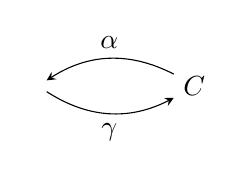
\begin{tikzpicture}[->, >=stealth]
    % Nodes
    \node (A) at (0,0) {\(\bA\)};
    \node (C) at (2,0) {\(\mathbb{C}\)};
    
    % Arrows
    \path
    (C) edge[bend right=30] node[above]{$\alpha$} (A)
    (A) edge[bend right=30] node[below]{$\gamma$} (C);
  \end{tikzpicture}
  \caption{Galois connection between an abstract domain \(\bA\) and a
    concrete domain \(\mathbb{C}\)}\label{fig:one}
\end{figure}